
\documentclass[9pt,xcolor={svgnames}]{beamer}

\mode<presentation> {
\usetheme{default}
\usepackage{makecell}
\usepackage{threeparttable}  
\usepackage[normalem]{ulem}

\usepackage{tikz}
\usepackage{colortbl} % For coloring cells
\usepackage{pgfplots}
\pgfplotsset{compat = newest}
\usetikzlibrary{positioning, arrows.meta}
\usepgfplotslibrary{fillbetween}

\usetikzlibrary{positioning, arrows.meta}
\usepackage{natbib}
\usepackage{soul}
\usepackage{cancel}

\usepackage{graphicx}

\bibliographystyle{plainnat}



%\setbeamertemplate{footline} % To remove the footer line in all slides uncomment this line
\setbeamertemplate{footline}[frame number] % To replace the footer line in all slides with a simple slide count uncomment this line
\setbeamertemplate{footline}
{
  \hfill%
  \usebeamercolor[fg]{page number in head/foot}%
  \usebeamerfont{page number in head/foot}%
%  \insertframenumber\,/\,\inserttotalframenumber\kern1em\vskip2pt % original code
  \tiny % font size: tiny(default)/scriptsize/footnotesize/small/normalsize/large
  \insertframenumber
  \kern1em  % adjust the space on the right-hand side of the frame number
  \vskip4pt % adjust the space below the frame number
}

\setbeamertemplate{navigation symbols}{} % To remove the navigation symbols from the bottom of all slides uncomment this line
}

\usepackage{graphicx} % Allows including images
\usepackage{booktabs} % Allows the use of \toprule, \midrule and \bottomrule in tables
\usepackage{multicol}
\usepackage{mathtools}
\usepackage{geometry}
\usepackage{bbm}

\usepackage[export]{adjustbox}


\setbeamertemplate{caption}[numbered]
\setbeamertemplate{itemize items}[circle]
\setbeamertemplate{itemize subitem}[default]
%\setbeamertemplate{enumerate items}[circle]\\
%\setbeamertemplate{items}[circle]

%\setbeamercolor{item}{fg=black} % all frames will have bullets with this color
%\setbeamercolor{caption name}{fg=gray} % all frames will have captions with this color

\usefonttheme[onlymath]{serif}

\setlength{\leftmargini}{9pt}
\setbeamersize{text margin left=20pt,text margin right=20pt}
%\setbeamerfont{institute}{size=\normalsize}

\setbeamertemplate{frametitle}
{
{\vskip  .6em} 
{\hskip -.35em}
\underline{\insertframetitle\vphantom{j}}
{\vskip -.6em}
}

\graphicspath{{./figs181007/}}


%----------------------------------------------------------------------------------------
%   TITLE PAGE
%----------------------------------------------------------------------------------------

\title[Bridging the Manufacturing Gap]{\large \textbf{Coordinating Skill Demand and Supply\footnote{The views in the presentation are the authors' own, not necessarily those of the IMF, its Executive Board, or management.}\\ %\normalsize A search-and-matching view of industrialization and the manufacturing gap
}
}

\addtobeamertemplate{title page}{%
  \begin{tikzpicture}[remember picture,overlay]
    \node[anchor=north east, xshift=-0.15cm, yshift=-0.15cm]
      at (current page.north east)
      {
\includegraphics[height=1.5cm]{logo.png}};
  \end{tikzpicture}%
}{}


\author{Shisham Adhikari, UC Davis \\  %\thanks{University of California – Davis; \texttt{shadhikari@ucdavis.edu}} 
\vspace{3mm}
\and Si Guo, Western Hemisphere Department,  IMF}    %\thanks{International Monetary Fund; \texttt{sguo@imf.org}}}

\date[Davis]{%
%  UC Davis Development Tea\\[0.5em]
  \today
}

\begin{document}

\begin{frame}
\titlepage % Print the title page as the first slide
\end{frame}

    %===============================================


\section{Past} 
\begin{frame}{Motivation: A Circular challenge about skill shortage}\label{main:intro}

% tighten the space between columns
\setlength{\columnsep}{8pt}

\begin{columns}[T,onlytextwidth]
% ---- Left: text ----
\begin{column}{0.62\textwidth}
 \begin{itemize}

  \item \textbf{Renewed interest in  manufacturing,} 
    %many of them also cover STEM education and training.
    \begin{itemize}
        \item China, US, Korea ...: industrial policy initiatives
        \item Many EMs: premature de-industrialization
    \end{itemize}

\vspace{2mm}
 
    \item \textbf{Circular challenge about skill shortage} 
    \begin{itemize}
        \item Firms report a shortage of appropriately skilled workers. \hyperlink{app:media}{\beamerbutton{Media}}

        \item Workers report a lack of industrial jobs and low pay perspectives. \hyperlink{app:jobshort}{\beamerbutton{EU survey}}

    \end{itemize}
    
    \vspace{4mm}

    \item This circular pattern raises questions about market failures and policy intervention. If yes, where should policy act (on firms? on workers' training?)
    
    \vspace{4mm}
    
  
  \end{itemize}
\end{column}

% ---- Right: tight cycle chart ----
\begin{column}{0.38\textwidth}
\vspace*{6mm} % push the figure down a bit
\begin{tikzpicture}[
  >=Latex,
  every node/.style={font=\scriptsize, text=structure.fg},
  line width=0.9pt,
  baseline
]
  % radii: arrows (R) and labels (T)
  \def\R{1.05}
  \def\T{1.60}

  % arrows (clockwise)
  \draw[->, draw=structure.fg] (180:\R) arc[start angle=180, end angle=90,  radius=\R];
  \draw[->, draw=structure.fg] ( 90:\R) arc[start angle=90,  end angle=0,   radius=\R];
  \draw[->, draw=structure.fg] (  0:\R) arc[start angle=0,   end angle=-90, radius=\R];
  \draw[->, draw=structure.fg] (-90:\R) arc[start angle=-90, end angle=-180,radius=\R];

  % labels
  \node[yshift=-1.2mm] at (90:\T)  {firms struggle to recruit};
  \node[xshift=1mm]     at (  0:\T)  {Fewer firms};
  \node[yshift=1.2mm]   at (-90:\T)  {Less value to workers};
  \node[xshift=-2mm]    at (180:\T) {Fewer workers};
\end{tikzpicture}

\begin{flushright}
  {\tiny\emph{Chicken-and-egg cycle in manufacturing expansion}}
\end{flushright}
\end{column}
\end{columns}

\vspace{4mm}
\small
%\textit{This paper formalizes this circular pattern in a two-sector search-and-matching labor model.}

\end{frame}


% ===================== WHAT DO WE DO =====================
\begin{frame}{What do we do?}\label{main:summary1}
\begin{itemize}

  \item \textbf{Model}

  Search frictions as in \textcolor{blue}{Acemoglu-Shimer (1999)} + two sectors + open economy 

\vspace{2mm}

\item \textbf{Key assumption/mechanism}

\begin{itemize}
    \item "Capital holdup" + wage bargaining: 
    
    Sunk investment  weakens firms' bargaining position and hence reduces investment return and job creation.
    It affects manufacturing more due to higher capital intensity. 
\end{itemize}

\vspace{2mm}

 % \item \textbf{Question}
 % \begin{itemize}
 %     \item Should governments actively support manufacturing and/or STEM education?
 %     \item If yes, \textbf{where} should policy act? On firms’ investment? On workers’ training?
 % \end{itemize}
 % \vspace{2mm}
  \item \textbf{Findings}
    \begin{itemize}
      \item If \textit{Hosios condition} holds,\footnote{Hosios condition is a technical condition that ensure private returns to job creation equals social returns in labor search models.} optimal policy only acts on firm's side:
      \begin{itemize}
    %      \item Capital holdup affects investment and job creation (and more so in manufacturing). 
          
          \item Investment subsidy (or CIT cut) financed by a "headcount" tax on firms, {fiscally neutral}. %and   \textbf{no need to intervene on workers' side.}
      \end{itemize}

\vspace{2mm}
      
      \item If the Hosios condition does \textit{not} hold, % e.g., workers' bargaining power is too small,
        \begin{itemize}
          \item A new wedge distorts' workers sectoral choices.
          \item {Needs interventions on  both sides of the labor market.}
       
      \end{itemize}

      \vspace{2mm}

   %       \item More service trade openness also boosts manufacturing employment. 
    \end{itemize}
\end{itemize}


\hyperlink{app:cardullo}{\beamerbutton{Holdup evidence}}


\end{frame}





% ===================== HOW DO WE DO IT =====================

%\begin{frame}{Outline}
%\begin{itemize}
%    \item \textbf{Empirics:}  
%    Cross-country patterns in STEM enrollment and industry employment

  %  \medskip

  %  \item \textbf{Theory:}  
  %  A two-sector model (manufacturing $m$ and services $s$) 
  %  with search frictions and endogenous capital
%  \medskip

%    \begin{itemize}
%        \item Inefficiency: decentralized equilibrium (DE) vs. social planner (SP)
 %       \vspace{2mm}


  %     \end{itemize} 
  %     \item Quantitative exercise
  %     \begin{itemize}
    
  %      \item Policy mapping and calibration to an “average” emerging market (EM)
%\vspace{2mm}
%        \item How service openness affects labor market outcome in manufacturing.  
 %   \end{itemize}
 %      \end{itemize}
%\end{frame}

\begin{frame}{Relations to literature}

\begin{itemize}
    \item \textbf{Labor search.}   Extend \textcolor{blue}{AS1999} to a \emph{two‐sector} environment (manufacturing vs. services) with international trade and sector‐specific capital intensity; calibrated to a manufacturing–services context. Also related to \textcolor{blue}{Cardullo et al. (2015)} and \textcolor{blue}{Grout (1984)} on capital holdup and \textcolor{blue}{Acemoglu (2001)} on labor market sectoral composition.

    \medskip

    \item \textbf{Structural change.} Most studies   characterize manufacturing shares under frictionless environment, with only a few exceptions (e.g., \textcolor{blue}{Feng et al. (2024)}). % We explore how labor frictions with capital holdup  shapes  policy rankings.

\medskip

    \item \textbf{Industrial policy}.  Complementary to studies built on manufacturing's increasing return to scale (\textcolor{blue}{Matsuyama (1991)}) or production network centrality (\textcolor{blue}{Liu (2019)}), our channel operates through labor‐market frictions within an otherwise standard framework.
\end{itemize}

%\vspace{1em}
%\textbf{Main contribution:} Two sectors + SOE + endogenous capital + education choice → three sources of inefficiency; Take labor market frictions seriously. 
\end{frame}


\begin{frame}{Tertiary enrollment by field varies a lot by country, 2019}\label{threecountry}
\begin{center}
%\textbf{\large Higher Education Enrollment Distribution by Fields}

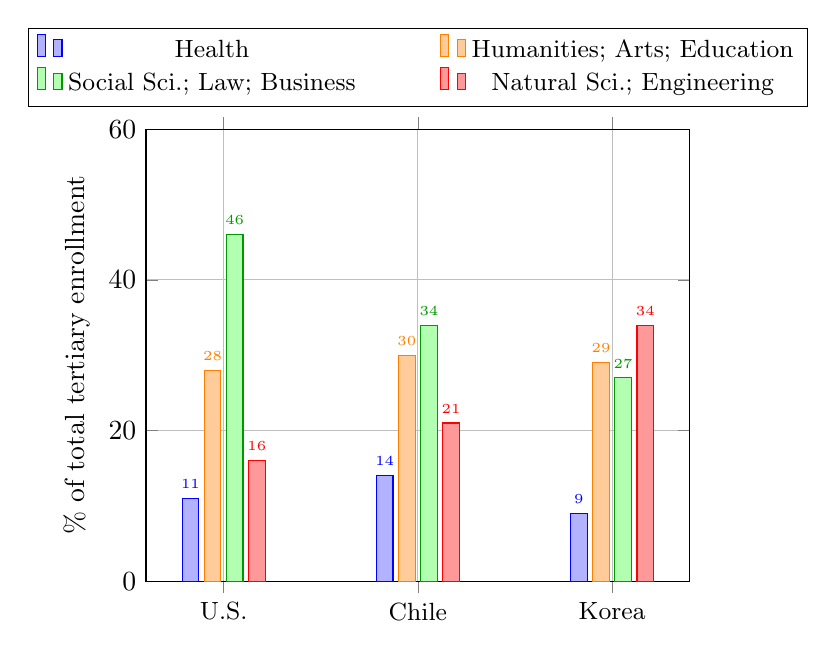
\begin{tikzpicture}
\begin{axis}[
    width=0.7\linewidth,
    ybar,
    bar width=6pt,
    ylabel={$\%$ of total tertiary enrollment},
    symbolic x coords={U.S., Chile, Korea},
    xtick=data,
    ymin=0,
    ymax=60,
    enlarge x limits=0.2,
    legend style={
        at={(0.5,1.05)},
        anchor=south,
        legend columns=2,
        font=\small,
        /tikz/every even column/.append style={column sep=1cm}
    },
    grid=major,
    nodes near coords,
    every node near coord/.append style={font=\tiny},
    ymajorgrids=true,
    xticklabel style={font=\small},
]

% Health (blue)
\addplot+[style={blue,fill=blue!30}] coordinates {
    (U.S.,11) (Chile,14) (Korea,9)
};

% Humanities, Arts, Education (orange)
\addplot+[style={orange,fill=orange!40}] coordinates {
    (U.S.,28) (Chile,30) (Korea,29)
};

% Social Sci., Law, Business (green)
\addplot+[style={green!60!black,fill=green!30}] coordinates {
    (U.S.,46) (Chile,34) (Korea,27)
};

% Natural Science, Engineering (red)
\addplot+[style={red,fill=red!40}] coordinates {
    (U.S.,16) (Chile,21) (Korea,34)
};

\legend{
    Health, Humanities; Arts; Education,
    Social Sci.; Law; Business, Natural Sci.; Engineering
}
\end{axis}
\end{tikzpicture}
\end{center}

\begin{center}
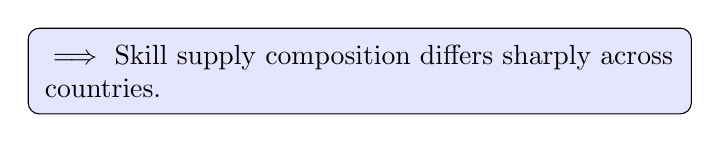
\begin{tikzpicture}
    \node[
        draw,
        rectangle,
        rounded corners,
        fill=blue!10,
        text width=8cm,
        align=left,   % <-- left-align text and let it fill the width
        inner sep=6pt
    ] (box) {
        $\implies$ Skill supply composition differs sharply across countries.
    };
\end{tikzpicture}
\end{center}


%\hyperlink{main:scatterplot}{\beamerbutton{Go back}}




\end{frame}





\begin{frame}{Skill demand and supply move together.}\label{main:scatterplot}
\begin{figure}[htbp]
    \centering
    \caption{STEM share vs. industrial employment share, 2019.}
    \label{fig:stem_ind}
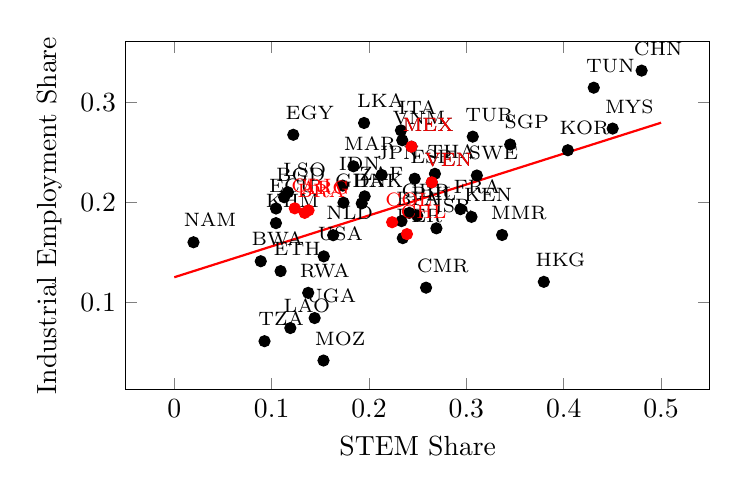
\begin{tikzpicture}
  \begin{axis}[
    width=9cm,
    height=6cm,
    % title={Relationship between STEM Share and Industrial Employment},
    xlabel={STEM Share},
    ylabel={Industrial Employment Share},
    ytick distance=0.1,  
    enlargelimits=0.1,
    scatter/classes={
        a={mark=o,draw=blue}
    },
    every node near coord/.append style={font=\scriptsize} % smaller font for country labels
  ]

    % Scatter points with country names as labels
  \addplot[
  scatter,
  only marks,
  scatter src=explicit symbolic,
  nodes near coords,
  nodes near coords align={center},
  nodes near coords style={font=\scriptsize, yshift=8pt, xshift=6pt} % shift label above marker
]
    coordinates {
 %(0.1378744,0.1921153)[ARG]
  (0.2333404,0.1812904)[BFA]
  (0.1127611,0.2052854)[BGD]
 % (0.1339324,0.1895628)[BRA]
  (0.0887872,0.1410377)[BWA]
 % (0.2389722,0.1682635)[CHL]
  (0.48,0.3322481)[CHN]
  (0.2586084,0.1145408)[CMR]
 % (0.223719,0.1801721)[COL]
 % (0.1237097,0.194118)[CRI]
  (0.1925061,0.1990896)[DNK]
  (0.1045007,0.193951)[ECU]
  (0.122197,0.2678931)[EGY]
  (0.2469077,0.223834)[ESP]
  (0.1091694,0.1311437)[ETH]
  (0.2938787,0.1932734)[FRA]
  (0.2413404,0.1895179)[GBR]
  (0.1737703,0.1997761)[GHA]
  (0.3795342,0.1203752)[HKG]
  (0.1730061,0.2169031)[IDN]
  (0.2692143,0.1740516)[ISR]
  (0.2328073,0.2722787)[ITA]
  (0.213,0.2275904)[JPN]
  (0.3052545,0.1855444)[KEN]
  (0.104402,0.1792649)[KHM]
  (0.4042146,0.2523832)[KOR]
  (0.1191805,0.0740409)[LAO]
  (0.1948983,0.2797219)[LKA]
  (0.116723,0.2102498)[LSO]
  (0.1840243,0.2362694)[MAR]
  (0.2436201,0.2559769)[MEX]
  (0.336678,0.1673723)[MMR]
  (0.1532314,0.0414321)[MOZ]
  (0.4502603,0.2741223)[MYS]
  (0.0197044,0.1600689)[NAM]
  (0.1631535,0.1671708)[NLD]
  (0.2346783,0.1642373)[PER]
  (0.2495234,0.1866893)[PHL]
  (0.1375139,0.1093415)[RWA]
  (0.3450148,0.2581424)[SGP]
  (0.3107809,0.2270485)[SWE]
  (0.2676974,0.228728)[THA]
  (0.4308376,0.3151194)[TUN]
  (0.3065551,0.2660213)[TUR]
  (0.0926554,0.0608464)[TZA]
  (0.1441461,0.0840602)[UGA]
  (0.1535388,0.1459264)[USA]
  (0.2644799,0.2202186)[VEN]
  (0.2341544,0.2624081)[VNM]
  (0.1955149,0.206129)[ZAF]
};


\addplot[
  scatter,
  only marks,
  scatter src=explicit symbolic,
  point meta=explicit symbolic,
  mark=*,
  mark options={draw=red, fill=red},
  nodes near coords={\pgfplotspointmeta},
  nodes near coords align={center},
  nodes near coords style={font=\scriptsize, yshift=8pt, xshift=6pt, text=red}
]
coordinates{
  (0.1378744,0.1921153)[ARG]
  (0.1339324,0.1895628)[BRA]
  (0.2389722,0.1682635)[CHL]
  (0.223719,0.1801721)[COL]
  (0.1237097,0.194118)[CRI]
  (0.2436201,0.2559769)[MEX]
  (0.2644799,0.2202186)[VEN]
};

  
    

    % Trend line (replace slope/intercept with your regression results)
    \addplot[red, thick, mark=none, domain=0:0.5] {0.31*x + 0.125};
   % \addlegendentry{Trend line (yhat)}

  \end{axis}
\end{tikzpicture}

    \begin{minipage}{0.7\textwidth}  % Adjust width to match figure
        \footnotesize
        \textbf{Note:} STEM share is calculated as the annual number of tertiary graduates in STEM fields divided by total number of tertiary graduates. Industrial employment share is calculated as the number of employees in the industry sector divided by total employment.
    \end{minipage}
    
\end{figure}

\hyperlink{app:datasource}{\beamerbutton{Data source}}
\hyperlink{app:regression}{\beamerbutton{Regression}}
%\hyperlink{threecountry}{\beamerbutton{Example}}

\end{frame}








\begin{frame}{Model: preferences and prices}\label{main:preference}
  \begin{itemize}
    \item \textbf{Final consumption} is a composite of manufacturing  and services consumption:
      \begin{align*}
                  C = C_m^{\alpha}C_s^{1-\alpha}
      \end{align*}
    
    \vspace{2mm}
%\item Elasticity of substitution $\sigma = 1/(1-\rho) <1$, so $m$ and $s$ are \textbf{complements}. 
\medskip
    \item Let final good be numeraire $P=1$, relative prices satisfy
    \begin{align*}
             p_m &= \alpha\,C_m^{-1}C, \\
        p_s &= (1-\alpha)C_s^{-1}C
    \end{align*}

\item Market clearing. Investment uses manufacturing goods. 

\begin{align*}
    C_m &= Y_m - I\\
    C_s & = Y_s
\end{align*}
where $I$ is capital investment for creating new vacancies (to be elaborated later).
   
%\item Continuous time, infinite horizon; discount rate $r$.
  \end{itemize}



\hyperlink{app:proof}{\beamerbutton{Go to Appendix}}

  
\end{frame}



\begin{frame}{Key mechanism}


\begin{itemize}
    \item Frictionless labor market:    $K^*_i, L^*_i$ are (efficiently) determined by
    \begin{align*}
 L^*_m:  \quad \quad  p_m   F_L(K_m, L_m) &= w = p_sF_L(K_s, L-L_m)   \\
  K^*_i: \quad  \quad    p_m F_K(K_m, L_m) & =r = p_sF_K(K_s, L-L_m)  
    \end{align*}

\item With search frictions + capital holdup
\begin{align*}
 L^*_m:  \quad     J_m(w_m, \theta_m ; p_m, K_m, L_m) & = J_s(w_s, \theta_s; p_s, K_s, L-L_m)  \\
  K^*_i: \quad  \quad   \quad \quad \quad    p_m F_K(K_m, L_m) & \neq r \neq p_sF_K(K_s, L-L_m)  
\end{align*}



\textbf{when $K^*_i$ is inefficiently small due to capital holdup (and more so in manufacturing), $L^*_m$ is inefficiently small.}
    
\end{itemize}
    
\end{frame}



\begin{frame}{Production in sector $i=m,s$}
  \begin{itemize}
    \item \textbf{Each job is a one plant-one worker match.} %Output of each match depends on technology $A_i$ and per-plant capital $k_i$
      \[
        y_i  =  f_i(k_i)  =A_i k_i^{a_i}
      \]
     % where $\bar{c}_s > 0$ is subsistence consumption of services.
    
    % \textcolor{red}{Let's use these notations consistently: $A_i$ is within $f_i$. Replace $\phi_i$ with $f_i$, also $f$ always has a substript. I corrected a lot but there could be some places omitted }
      \medskip
      \item \textbf{Manufacturing is more capital intensive than services}: $a_m > a_s$.
    
    
    \medskip
    \item \textbf{Sectoral output}
      \begin{align*}
       Y_i = y_i \cdot  \underbrace{(L_i-u_i)}_{\text{employment in i}},
      \end{align*}
   %   with $L_a$ exogenous.
    \medskip
 %   \item \textbf{Total labor force is fixed, but sectoral composition $\{L_m, L_s\}$ is endogenous:}
  %    \[
  %      L_m+L_s =L
  %    \]

   \item \textbf{Two skill tracks:} STEM (cost $\epsilon_m$) vs.\ Non‐STEM (cost $\epsilon_s$) 
      \[
       % \text{Cost: } \epsilon_h ;  \epsilon_l,\quad
        \text{STEM} \to \text{search in sector }m ,\quad \quad 
        \text{Non‐STEM} \to \text{search in sector }s.
      \]

 \begin{align*}
     L_m+L_s=L
 \end{align*}

 
  \end{itemize}
\end{frame}





\begin{frame}
\frametitle{Labor markets are segmented with standard DMP frictions}
\vspace{1em}
 \begin{itemize}

  


    \vspace{1em}

\item  \textbf{Firms create vacancies}.

   $k_i$: upfront investment for each vacancy.

  $x_i$: newly created vacancies, some will be matched with workers, some will stay idle.


    $s_i$: exogenous probability that a vacancy is destroyed. \\

  \vspace{3mm}

    
    \item \textbf{Search \& Matching}:    
      
  $ u_i$ and $v_i$:   \quad number of unemployed and vacancies in sector $i$\\
  \vspace{1mm}
    $ M(u_i,v_i)$: \quad \text{the flow of job matches}  \\
\vspace{1mm}
       $ \theta_i \;=\; \frac{v_i}{u_i}$: \quad  labor market tightness \\
       \vspace{1mm}
       $ q_i(\theta_i) \;=\; \frac{M_i(u_i,v_i)}{v_i}$: \quad  firms' vacancy filling rate\\
       \vspace{1mm}
      $  \theta_i\,q_i(\theta_i) \;=\;\frac{M_i(u_i,v_i)}{u_i}:$ \quad 
      workers' job finding rate \\


\vspace{1mm}
      \vspace{1mm}
      
  %   \item \textbf{Steady‐state unemployment/ Beveridge curve:}
   %   \[
   %     u_i \;=\; \frac{s_iL_i}{\,s_i + \theta_i\,q_i(\theta_i)\,}, 
   %     \quad i\in\{m,s\}.
   %   \]
       

         \vspace{5mm}

%\item    Unemployment and vacancy dynamics
%   \begin{align*}
%       d u_i/d t & = s_i(L_i-u_i) - M(u_i, v_i) \\
%              d v_i/d t & = x_i - M(u_i, v_i) -s_iv_i
%   \end{align*}




\item \textbf{Investment.} Firms decides to capital levels $k_m, k_s$ when they create vacancies. 

Total investment flow $I = x_mk_m + x_sk_s$.
  \end{itemize}
\end{frame}






\begin{frame}{Bellman equations}
%\textit{Intuition:} Each $J$ is a \emph{lifetime value} (present discounted value) of a state.
%$rJ = \text{current payoff} + \text{expected change}.$


%\textit{Key assumption:} 


\vspace{1em}
  \begin{itemize}


   \item \textbf{To create a vacancy, firm needs to make (sunk) investment $P_k k_i$. }
\[
 Profit_i= Max_{\{k_i\}}  \quad J^V_i(k_i)  \textcolor{blue}{- P_kk_i}
\]

  
  \item \textbf{Firm Value Functions:}
     \[
      \begin{aligned}
           rJ_i^V(k_i) &=  q_i(\theta_i)\big(J_i^F(k_i)-J_i^V(k_i)\big) - \textcolor{blue}{s_i J^V_i(k_i)} \\
             rJ_i^F(k_i) &= p_i f_i(k_i) - w_i(k_i) - s_i J_i^F(k_i)
     %    k_i^*&= argmax_{k_i} \{ J_i^V(k_i) - P_kk_i \} \\
      \end{aligned}
\]
  
    \item \textbf{Worker Value Functions:}
      \[
      \begin{aligned}
        rJ_i^U &= z+ \theta_i q_i(\theta_i)\big(J_i^E(k^*_i)-J_i^U\big),\\
        rJ_i^E(k_i) &= w_i(k_i) + s_i\big(J_i^U-J_i^E(k_i)\big), \\
      \end{aligned}
   %   \quad i\in\{m,s\}.
      \]
  
      
      
    \item \textbf{Wage Bargaining:}
      \[
        (1-\beta)\bigl(J^E_i(k_i) - J^U_i\bigr)
        = \beta\bigl(J^F_i(k_i) - J^V_i(k_i)\bigr)\
        %;\Rightarrow\;
       % w_i = \beta\,(p_i - r\,k_i) + (1-\beta)\,r\,J^U_i.
      \]

    \item \textbf{Workers decide which sector to enter:}
\[
 \textcolor{blue}{  J^U_m  - J^U_s  = \epsilon_m - \epsilon_s}
\]


%\quad \quad \quad \quad \quad \quad  In equilibrium $Profit_i = 0$.
      
  \end{itemize}
\end{frame}




\begin{frame}{Hosios condition $\beta=\eta$}


$\beta$: worker's bargaining power

$\eta$: elasticity of matching function $M(u, v) = u^{\eta}v^{1-\eta}$.

\vspace{4mm}


Search externalities: when firm creates one more vacancy, it only accounts for his private return $(1-\beta)qS$, ignoring that this one more vacancy can affect overall market tightness $\theta$. 

\vspace{2mm}



\begin{itemize}
    \item Private return from a vacancy: $(1-\beta) q S$

\item Social return from a vacancy: $(1-\eta)q S$
\end{itemize}


\vspace{3mm}
 $\rightarrow$ Hosios condition $\beta=\eta$ kills search externalities.
\end{frame}



\begin{frame}{Decentralized Equilibrium vs Social Planner}
\small
\vspace{2mm}
\begin{columns}[T,onlytextwidth]
% ---------------- Left: DE ----------------
\begin{column}{0.485\textwidth}
\textbf{Decentralized Equilibrium (DE)}
\vspace{0.3em}

\textbf{1. FOC wrt $k_i$:}
\[
P_k =\textcolor{red}{ (1-\beta)}\cdot
\frac{p_i f_i'(k_i)}{r+s_i}\cdot
\frac{q_i(\theta_i)}{r+s_i+(1-\beta)q_i(\theta_i)}
\]

\vspace{-0.3em}\hrule\vspace{0.6em}

\textbf{2. Free-entry condition:}
\[
P_k k_i = (1-\textcolor{red}{\beta})\, q_i(\theta_i)\,\frac{1}{r+s_i}\, S_i
\]

\vspace{-0.3em}\hrule\vspace{0.6em}

\textbf{3. Educational choice:}
\[
r(\epsilon_m-\epsilon_s)=\textcolor{red}{\beta}[\theta_m q_m(\theta_m) S_m
-\theta_s q_s(\theta_s) S_s]
\]
\end{column}

% -------- Vertical divider in the middle --------
\begin{column}{0.03\textwidth}
\centering
\rule{0.4pt}{0.78\textheight}
\end{column}

% ---------------- Right: SP ----------------
\begin{column}{0.485\textwidth}
\textbf{Social Planner (SP)}
\vspace{0.3em}

\textbf{1. FOC wrt $k_i$:}
\[
P_k = 
\frac{p_i f_i'(k_i)}{r+s_i}\cdot
\frac{q_i(\theta_i)}{r+s_i+q_i(\theta_i)}
\]

\vspace{-0.3em}\hrule\vspace{0.6em}

\textbf{2. Free-entry condition:}
\[
P_k k_i = (1-\textcolor{red}{\eta})\, q_i(\theta_i)\,\frac{1}{r+s_i}\, S_i
\]

\vspace{-0.3em}\hrule\vspace{0.6em}

\textbf{3. Educational choice:}
\[
r(\epsilon_m-\epsilon_s)=\textcolor{red}{\eta}[\theta_m q_m(\theta_m) S_m
-\theta_s q_s(\theta_s) S_s]
\]


\vspace{8mm}
 $\eta$: parameter in  $M(u,v)=u^\eta v^{1-\eta}$.

$\beta$: workers' bargaining weight.

 $S_i$: matching surplus in sector $i$.

 $\epsilon_i$: training costs in sector $i$

 $P_k$: capital price
 
\end{column}
\end{columns}

\vspace{5em}
%\textcolor{blue}{\textbf{Key wedge}}\\
%{\small Holdup/bargaining replaces the planner’s $(1-\eta)$ and $\eta$ with $(1-\beta)$ and $\beta$.
%With capital intensity higher in $m$, the induced distortion in $k_m$ (hence $\theta_m,q_m,L_m$) is larger.}




\end{frame}













%\begin{frame}{Efficiency: Under Hosios only capital underinvestment inefficiency matters}
%If Hosios condition $\eta = \beta$ holds %\footnote{Hosios insight: the efficient allocation weight each side of the market according to how much it contributes to match formation, not according to bargaining strength.},
%\begin{itemize}
%   \item Wedge between DE vs. SPP, reflecting capital hold-up problem
%\[
%\frac{\text{Marginal K return}^{DE}}{\text{Marginal K return}^{SP}}
%\;=\;(1-\beta_i)\,\frac{\,r+s_i+q_i(\theta_i)\,}{\,r+s_i+(1-\beta_i)\,q_i(\theta_i)\,}.
%< 1\]
%\[k^{DE} < k^{SP}.\] 

%\item No wedges between DE and SPP in tightness and sectoral choice conditions!

%\end{itemize}


%\vspace{0.1cm}
%\begin{center}
%\begin{tikzpicture}
%    \node[
%        draw,
%        rectangle,
%        rounded corners,
%        fill=blue!10,
%        text width=10cm,
%        align=left,   % <-- left-align text and let it fill the width
%        inner sep=6pt
%    ] (box) {
%        $\implies$ Under Hosios, only the holdup problem remains, so policy should target firms only.
%    };
%\end{tikzpicture}
%\end{center}
%\end{frame}


\begin{frame}{Implement SP with $\beta=\eta$ includes a fiscally neutral plan}

Two fiscal instruments:  capital subsidy $\tau^K_i$ and a tax  $\tau^T_i$ per unit of labor. 

\begin{align*}
\text{FOC wrt k}: \quad \textcolor{blue}{ (1-\tau^K_i)}    P_k & =  (1-\beta)\frac{p_i\,f_i'(k_i)}{r+s_i}\;
   \frac{q_i(\theta_i)}{\,r+s_i + q_i(\theta_i)\,}.\\
 \text{Tightness:} \quad \textcolor{blue}{ (1-\tau^K_i)}       P_{k}\,k_i  &=  (1-\beta) q_i(\theta) \frac{S_i(k_i)}{(r+s_i)}  - \textcolor{blue}{\tau^T_i}
%\qquad i \in \{m,s\}.
\end{align*}

\begin{center}
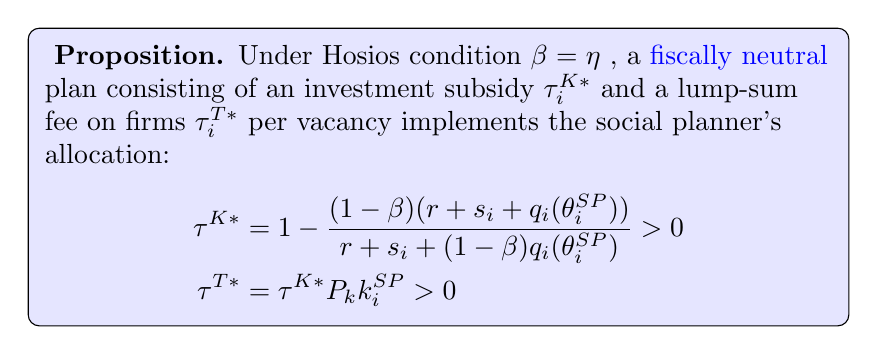
\begin{tikzpicture}
    \node[
        draw,
        rectangle,
        rounded corners,
        fill=blue!10,
        text width=10cm,
        align=left,   % <-- left-align text and let it fill the width
        inner sep=6pt
    ] (box) {
   \textbf{    Proposition.}     Under Hosios condition  $\beta=\eta$ , a \textcolor{blue}{fiscally neutral} plan consisting of an investment subsidy $\tau^{K*}_i$ and a lump-sum fee on firms $\tau^{T*}_i$ per vacancy implements the social planner's allocation:
       \begin{align*}
    \tau^{K*} & =  1-\frac{(1-\beta)(r+s_i+q_i(\theta_i^{SP}))}{r+s_i+(1-\beta)q_i(\theta_i^{SP})} >0\\
    \tau^{T*} & =  \tau^{K*}P_kk_i^{SP}>0
\end{align*}
    };
\end{tikzpicture}
\end{center}


Key takeaway: \textbf{When $\beta=\eta$, optimal policy is only on firm's side,  as skill supply composition will adjust endogenously once job creation is efficient.}

%\textbf{Key takeaway: when $\beta=\eta$, optimal  fiscally neutral investment subsidy financed by fee; no training subsidy needed.

%1. Only capital underinvestment matters. Once $k_i=k^{SP}$, skill composition $L_m$ will adjust endogenously to $L_m^{SP}$, and no need to subsidize training. 

%2. Optimal plan is fiscally neutral:  $k_i$-subsidy is fully financed by fees. 

    
\end{frame}


\begin{frame}{Evidence that skill supply catches up with skill demand}\label{app:oilshock}

Higher oil prices $\rightarrow$ higher petroleum  engineering  enrollment in  1970s and 2000s. 

\vspace{3mm}
     \centering
 % 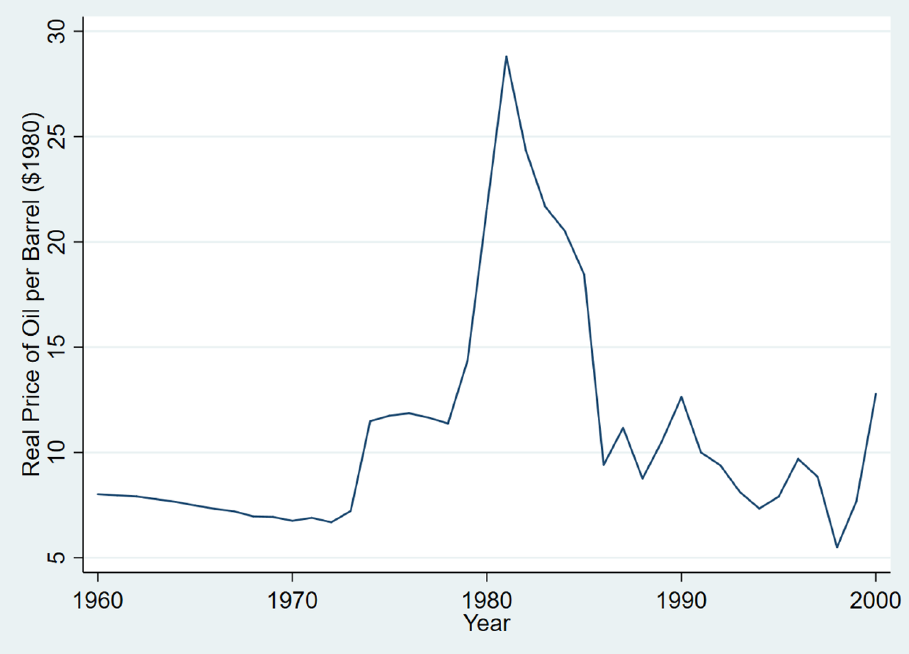
\includegraphics[width=0.45\textwidth]{han2.png}



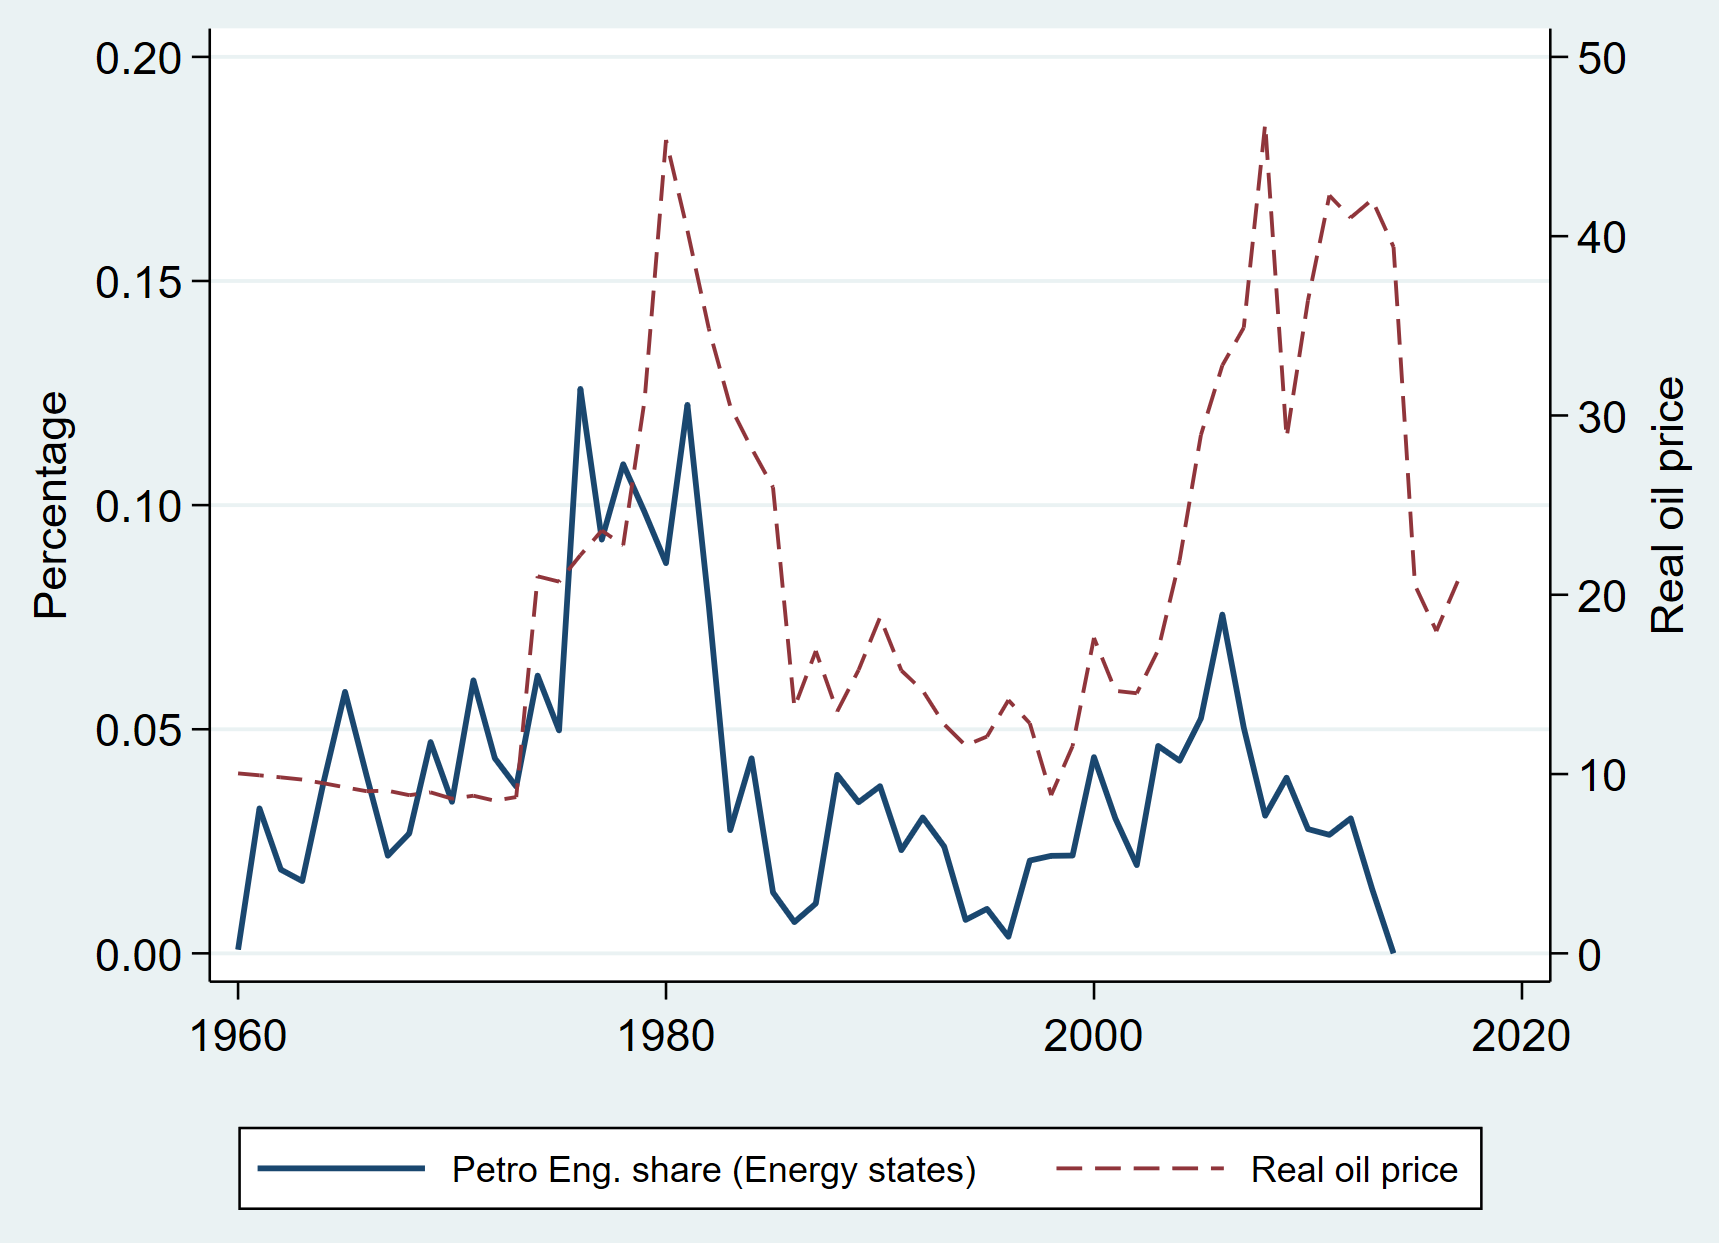
\includegraphics[width=0.7\textwidth]{oil_major.png}
% \centering
%  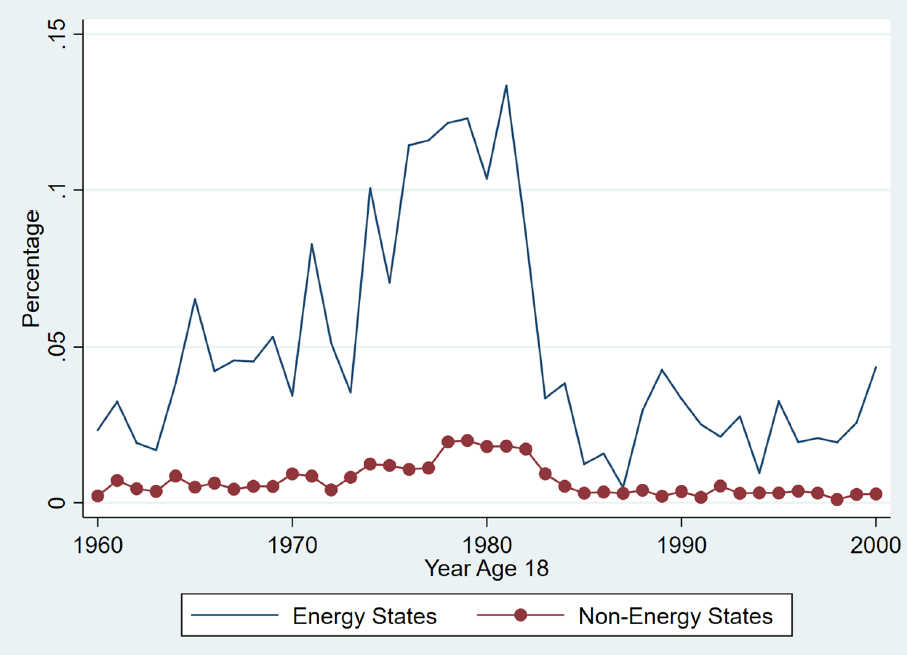
\includegraphics[width=0.45\textwidth]{han1.png}

\text{Data source: American Community Survey and Haver.}


 %    \hyperlink{main:conclusion}{\beamerbutton{Go back}}

\end{frame}


\begin{frame}{When Hosios fails, a new wedge distorts sectoral labor supply.}\label{main:beta_eta}


\begin{itemize}


\item $\beta< \eta$ could also be empirically relevant. \hyperlink{app:beta_eta}{\beamerbutton{Go to Appendix}}


%\item Deviation from Hosios condition affects $m$ and $s$ sectors \textbf{asymmetrically},  justifying the subsidy on $m$ sector workers' education/skills costs.\\

\vspace{5mm}

%    \item Additional need to 



    \item Comparing the sectoral choice conditions (after substituting tightness condition) in SP and DE: %RHSs measure workers' utility change from moving $s \rightarrow m$.

   % \begin{align*}
   %     r(\epsilon_m-\epsilon_s) &= \textcolor{red}{\eta} [\theta_mq_mS_m - \theta_sq_sS_s] \quad \text{(SP)}\\
   %      r(\epsilon_m-\epsilon_s) &= \textcolor{red}{\beta} [\theta_mq_mS_m - \theta_sq_sS_s]  \quad \text{(DE)}\\
   % \end{align*}

   \begin{align*}
    r(\epsilon_m-\epsilon_s) &= \textcolor{red}{\frac{\eta}{1-\eta}}[\theta_mP_kk_m(r+s_m)-\theta_sP_kk_s(r+s_s)]  \quad (\text{SP}) \label{rc_sp}\\
        r(\epsilon_m-\epsilon_s) &= \textcolor{red}{\frac{\beta}{1-\beta}}[\theta_mP_kk_m(r+s_m)-\theta_sP_kk_s(r+s_s)]  \quad (\text{DE}) \label{rc_de} 
\end{align*}

%   \item When entering $m$ is more costly ($ \epsilon_m -\epsilon_s >0$), workers need to collect more surplus from $m$ sector to compensate for the training cost difference.  But $\beta<\eta$ makes it difficult, leading to inefficiently low  $L_m$.

   % \item If we move from SP to DE, i.e., $\eta \rightarrow \beta$, workers in $m$ suffer a larger welfare loss than those in $s$ and will prefer entering $s$ sector more.  



When $\beta<\eta$, private returns undervalue sector $m$ entry relative to planner → too few workers train for sector $m$.
  %  $\rightarrow$ A wedge that distorts workers' choice when $\beta \neq \eta$. 
 %  This wedge \textcolor{blue}{differs} from Hosios: it exists even if $(\theta_i, k_i) = (\theta_i^{SP}, k_i^{SP})$.
\end{itemize}



\end{frame}




\begin{frame}{Policies implement SP when $\beta<\eta$ includes subsidy to training cost}
\small

\begin{center}
\begin{tikzpicture}
    \node[
        draw,
        rectangle,
        rounded corners,
        fill=blue!10,
        text width=10cm,
        align=left,   % <-- left-align text and let it fill the width
        inner sep=6pt
    ] (box) {



\textbf{Proposition.} Under $\beta<\eta$ and $\epsilon_m > \epsilon_s$, we can implement the SPP allocation using a triple of policy instruments $\{\tau^{K**}_i, \tau^{T**}_i, \tau^L_i^{**}\}$.


    };
\end{tikzpicture}
\end{center}

\begin{itemize}
    \item Investment subsidy to firms $\tau^K$: correct holdup/investment wedge

\item Headcount tax on firms $\tau^T$: correct vacancy/tightness externality

\item Training subsidy to workers $\tau^L$: correct sector-entry wedge 
\end{itemize}

    
\end{frame}



\begin{frame}{Quantitative exercise: add a trade block}\label{main:trade}
\paragraph{Preferences.}
\begin{align*}
    C &= C_m^{\alpha}C_s^{1-\alpha}
\end{align*}
$C_m$ is total output $Y_m$ subtracting export $X_m$
\begin{align*}
     C_m  = Y_m - X_m 
\end{align*}
$C_s$ is a CES composite of domestic and imported services.     
   \begin{align*}
    C_s &= [\chi (C_s^{H})^{\frac{\nu-1}\nu} + (1-\chi)\,(C_s^{F})^{\frac{\nu-1}{\nu}}]^{\frac{\nu}{\nu-1}}, 
   % P &= \alpha^{-\alpha}(1-\alpha)^{-(1-\alpha)}
\end{align*}

Investment uses $m$ goods:  
\begin{align*}
    I = P_k(x_mk_m + x_sk_s) 
\end{align*}

Balanced trade:  $p_m^F X_m = p_s^F C_s^F $

\textbf{Prices.}

Foreign prices are fixed:  $p_m^F = p_s^F = 1$. 

Domestic $m$ price $p_m$ has to equal foreign price $p_m^F$ due to perfect substitution.

Domestic services price $p_s$ is endogenous. 

\hyperlink{app:trade}{\beamerbutton{Trade equilibrium}}

    
\end{frame}


%===============================================
\section{Calibration and Results}
%===============================================

\begin{frame}{Calibration -- exogenous parameters}
    \begin{table}[h!]
\centering
\caption{Exogenously Set Parameters:}\label{table_set_parameters}
\begin{adjustbox}{width=0.8\columnwidth,center}
\begin{tabular}{||c c c c||}\hline
\textbf{Parameter} & \textbf{Description} & \textbf{Value} & \textbf{Source} \\\hline\hline
$\nu$ & CES aggregator coefficient & $2$ & Dimanranan et al. (2006) \\
$m$ & Matching efficiency & $1$ & Normalization \\
$\eta$ & Matching elasticity & $0.5$ & Petrongolo and Pissarides (2001) \\
$\beta$ & Worker bargaining weight & $0.5$ & Hosios condition \\
%$s_s$ & Service separation rate (annual) & $0.20$ & BLS/JOLTS \\
%$A_m$ & Manufacturing technology & $1$ & Normalization \\
$A_s$ & Services technology & $1$ & Normalization \\
$p_m$ & $m$ goods price & $1$  & Normalization  \\
$p_s^F$ & Foreign service goods price & 1 & Normalization 
%$\chi$ & Retirement (annual rate) & $0.025$ & 40-year working life 
\\\hline
\end{tabular}
\end{adjustbox}
\end{table}



\begin{table}[h!]
\centering
\caption{Internally Calibrated Parameters.}\label{table_calibrated_parameters}
\begin{adjustbox}{width=0.95\columnwidth,center}
\begin{tabular}{||c c c c||}\hline
\textbf{Parameter} & \textbf{Description} & \textbf{Value} & Data Moment \\\hline\hline
$\alpha$ & Preference weight on $m$ goods & $0.20$ & Industrial employment share \\
$s_m$ & Manufacturing separation rate (annual) & $0.047$ & Unemployment rate in $m$  \\
$s_s$ & Services separation rate (annual) & $0.115$ & Unemployment rate in $s$ \\
$\zeta_m$ & Capital share in manufacturing & $0.65$ & Capital share in $m$\\
$\zeta_s$ & Capital share in services & $0.3$ &  Capital share in $s$ \\
$r$ & Discount rate (annual) & $0.06$ & Capital-output ratio \\
$1-\chi$ & Service sector openness & 0.004 & Goods trade balance-to-GDP \\
$A_m/A_s$   & relative productivity & 2.0  &   sectoral wage ratio\\
$\epsilon_m-\epsilon_s$ & Education cost differential & 7.0 &  training cost differential/labor income \\ 
$z$  & Home production utility  & 3.0 & Home production-to-wage
\\\hline
\end{tabular}
\end{adjustbox}
\end{table}



\end{frame}


%\begin{frame}{Data targets and DE moments}


%\begin{table}[h!]
%\centering
%\caption{Matching the calibration targets and non-targeted moments.}\label{table_calibration_targets}
%\begin{adjustbox}{width=0.7\columnwidth,center}
%\begin{tabular}{||c c c||}\hline
%\textbf{Target} & \textbf{Data/Target} & \textbf{Model} \\\hline\hline
%Share of industrial employment, $L_m$ & $\sim 0.23$ & $0.23$ \\
%Unemployment rate ($m$)  & $\sim 7.0$ & $7.0$ \\
%Unemployment rate ($s$)  & $\sim 7.0$ & $7.0$ \\
%Capital-to-output ratio & $\sim 3.0$ & $3.0$ \\
%Labor income share ($m$)  & $0.36$ & $0.39$ \\
%Labor income share ($s$)  & $0.66$ & $0.75$ \\
%Goods trade surplus-to-GDP & $0.05$ &  $0.05$ \\
%Wage ratio $w_m/w_s$ & 1.04-1.14 & $1.09$  \\
%Training cost differential-to-wage & 0.7- 0.75 & 0.73 \\
%Home production-to-wage     & 0.25-0.35    &   0.31  
% & & \\  
%\textbf{Non-Targeted Moments} & & \\
%Capital formation-to-GDP & $0.23$ & $0.225$ 
%Aggregate unemployment rate & $0.06$–$0.10$ & $0.08$ 
%\\\hline
%\end{tabular}
%\end{adjustbox}
%\end{table}

    
%\end{frame}


\begin{frame}{Decentralized vs. Planner results }

\begin{table}[h!]
\centering
\caption{DE and SP Model Moments}
 \begin{tabular}{||c  c||} 
 \hline
 \textbf{Moments} &  \textbf{$\Delta$ from DE to SP} \\  
 \hline\hline
  Capital-to-output ratio, $K/Y$     &   +0.4\\
 % Total capital,  $K$  & 252  & 319 &  + 27\% \\
 % Relative prices, $p_s/p_m$ & 0.473  &  0.474 \\
%  Labor productivity, $A_m\f_m(k_m)/A_s\f_m(k_s)$ & 42.1 & 43.5 & $+3.3\% $\\ 
%  \textbf{Non-Targeted Moments} &  &  \\
% Relative wages, $w_m/w_s$ &  1.09 & 1.08 \\
 Output, $Y_m$  & +17.1\% \\
  Output $Y_s$  & +7.3\% \\
  Industrial labor force, $L_m$ &  +0.9 pp \\
  Industrial employment $n_m/(n+L_a)$  & +1.0 pp\\
  Industrial unemploy. rate, $u_m$ & +0.6 pp  \\ 
   Services unemploy. rate,  $u_s$  & +1.1 pp \\ 
 %  Total output $Y/P$  & +11.3\% \\
% Relative output, $Y_m/Y_s$ & 13.6  & 14.9  & $+1.3$\\
% Real output, $\sum p_iY_i/P$ &  84.4   &  93.9 & $+11.2\%$ \\
 % Training Expenses/GDP & 0.75\% & 0.75\% \\ 
 [1ex] 
 \hline
 \end{tabular}
%\end{adjustbox}
 
\end{table} 


\textbf{Key Takeaways}
\begin{itemize}
  \item  \textbf{Output gains of $~11\%$ from DE → SP,} driven primarily by $k_i \uparrow$
\medskip
         \item \textbf{Higher $L_m$ and $Y_m/Y_s$ in SP:} Both $k_m, k_s$ rise $\rightarrow$ labor productivity in $m$ rises more than $s$ due to higher capital intensity   $\rightarrow$ more workers choose $m$

          \item \textbf{Unemployment rates are higher in SP} -- $k_i \uparrow$ in SP $\rightarrow$ vacancy becomes more costly $\rightarrow$ and the number of vacancies $\downarrow$ and unemployment $\uparrow$  
         
         % Capital deepening improves labor productivity in $m$ sector more than $s$ sector; the efficient allocation uses more capital and fewer workers in $m$.
\end{itemize}
\end{frame}









\begin{frame}{When Hosios fails ($\beta<\eta$), tax/subsidy training is needed.}

Full package ($\tau^{K*}, \tau^{T*}, \tau^{L*}$) $\rightarrow$ replicates SP.

Partial package ($\tau^{K*}, \tau^{T*}$)   $\rightarrow$ lower $L_m$ and welfare than SP, reflecting the emergence of sectoral choice wedge. 


    
\begin{table}[H]
 %\caption{Equilibrium allocations, $\beta<\eta$} \label{policytable_small_beta}
\centering
\caption{\textbf{Change relative to DE, when $\beta=0.3< \eta=0.5$}}
\resizebox{\textwidth}{!}{
 \begin{tabular}{||c c  c||} 
 \hline
 \textbf{Moment}  & \textbf{Full Package}  & \textbf{Partial Package}\\  
 Description   & Implements SP  &  No training subsidy \\
%$\beta$    & 0.3  & 0.3  &  0.3 \\
%$\eta$   & 0.5  & 0.5  &  0.5 \\
  $\tau^K_i$   &  $\tau^K_i=\tau^{K**}_i$    &  $\tau^K_i = \tau^{K**}_i$  \\
    $\tau^T_i$      &  $\tau^T_i=\tau^{T**}_i$   &   $\tau^T_i=\tau^{T**}_i$  \\ 
        $\tau^L_m$      &  $\tau^L_m=\tau^{L**}_m$    &   0  \\ 
 \hline\hline
  Industry labor force, $L_m$  & \textcolor{black}{+$0.7$ pp}   & \textcolor{black}{  $-1.7$ pp} \\
  Industry unemp. rate, $u_m/L_m$  & $+2.9$ pp  &  $+2.5$ pp  \\ 
   Services unemp. rate, $u_s/L_s$  &  $+3.4$ pp   &   $+3.8$ pp  \\ 
  Capital-to-output ratio, $K/Y$    & +0.4  &  +0.4 \\
 % Tightness, $\theta_m$ & 0.41 & 0.95  &  0.34  &  0.39  \\
  %  Tightness, $\theta_s$ & 2.31 & 5.52 &  1.71  &  1.53 \\
  %Vacancy-filling rate, $q_m$ & 1.72 &   1.54   &  1.55 \\
  %  Vacancy-filling rate, $q_s$  & 0.76 &   0.64   &  0.65 \\
%  Total capital,  $K$  & 252  & 319 & $ + 27\% $\\
 % Relative prices, $p_s/p_m$ & 0.473  &  0.474 \\
%  Labor productivity, $A_m\f_m(k_m)/A_s\f_m(k_s)$ & 42.1 & 43.5 & $+3.3\% $\\ 
%  \textbf{Non-Targeted Moments} &  &  \\
% Relative wages, $w_m/w_s$ &  1.09 & 1.08 \\
 Real output, $Y_m$    & +15.3\%  & +3.2\%\\
 Real output, $Y_s$   & +8.0 \% &  +8.0\% \\
% Real consumption $C$   & 4.0 & 4.0  & 4.3  & 4.1  \\  
 %Welfare, $W$  &   4.1 & 4.0    &  4.4      &  4.3                      \\
 %Annual fiscal cost ($\%$ of GDP)  &   0   &  2.3  & 2.1 \\
 % Training Expenses/GDP & 0.75\% & 0.75\% \\ 
 \hline
 \end{tabular}}
%\end{adjustbox}
 
\end{table} 

\end{frame}




%===============================================
\section{Conclusion}
%===============================================
\begin{frame}{Conclusion}\label{main:conclusion}
\small
\begin{itemize}

\item A circular problem between firms' skill demand and workers' skill choice 

\medskip


 %\item In a search model with capital-intensive manufacturing, the decentralized equilibrium under-invests and yields an inefficiently small manufacturing sector.


\medskip
 \item  When Hosios  holds ($\beta=\eta$), firm-side policy only; skill supply follows.


 \medskip

 \item When Hosios fails ($\beta \neq \eta$),  training subsidy is also needed.


\medskip
\item Open economy: more service openness $\rightarrow$ $L_m \uparrow$ and $u_i  \downarrow$.  \hyperlink{app:open}{\beamerbutton{Open economy}}


%\medskip

%\item Premise of the paper: (at least when $\beta=\eta$) once skill demand composition adjusts, skill supply composition will catch up.  

%\vspace{2mm}


%Empirical support: the surge in oil price around 1980 in late 1970 lead to an increase in students enrolled in petroleum major. 

% \hyperlink{app:oilshock}{\beamerbutton{Oil shock}}


\end{itemize}


\end{frame}


\begin{frame}
  \centering
  \huge Thank you! \\
  \vspace{1em}
  \normalsize Questions?
\end{frame}


















%\appendix


%\begin{frame}[label=app:proof]{Appendix: Proof details}




\begin{frame}{Motivation: STEM skill shortages are reported across countries/industries.}\label{app:media}
  \begin{figure}
    \centering
    
\includegraphics[width=1\textwidth]{figures/employers.png}
    \label{fig:empirics}
  \end{figure}

\hyperlink{main:intro}{\beamerbutton{Go back}}

\end{frame}

\begin{frame}{Motivation: Workers concern  shortage of jobs}\label{app:jobshort}

\begin{itemize}



\item Surveys
\begin{itemize}
\item EU (2001, 2003): \textit{ "Young people are turning their backs on scientific careers, citing poor salary prospects as the chief reason. " }

\end{itemize}



\vspace{3mm}


    \item Students' major choices are affected by local labor market: \textcolor{blue}{Mather and Smith (2025)}, \textcolor{blue}{Conzelmann et al. (2023)},...
    
\end{itemize}

\hyperlink{main:intro}{\beamerbutton{Go back}}

%  \begin{figure}
%    \centering
%    
\includegraphics[width=1\textwidth]{figures/employees.png}
%    \label{fig:empirics}
%  \end{figure}
\end{frame}



\begin{frame}\label{app:cardullo}
\frametitle{Cardullo et al. (2015) -- empirical evidence on capital holdup}


For 11 OECD countries, run a regression 

\begin{align*}
    log (k_{i,c}) = \alpha (Sunk_i * Union_c) + Controls 
\end{align*}

$\alpha<0$ implies countries with stronger union coverage has lower capital per worker in industries with higher sunk capital. 

\hyperlink{main:summary1}{\beamerbutton{Go back}}

\end{frame}





\begin{frame}\label{app:datasource}
\frametitle{Data Source for the Stylized Empirical Motivation}
\begin{itemize}

\item \textbf{UNESCO (UIS):} Tertiary enrollment by field, 1999–2023. 
STEM = \textbf{ICT, Natural Sciences, and Engineering}.  
For each country, we take the \textbf{earliest available year} to approximate \textbf{initial STEM supply}.

\medskip

\item \textbf{Groningen Growth and Development Centre (GGDC, 10-sector / Structural Change):} 
Employment and value added, latest available year (2018 for most; 2011 for some).  
“\textbf{Industry}” $=$ mining $+$ utilities $+$ manufacturing $+$ construction.

\end{itemize}

\hyperlink{main:scatterplot}{\beamerbutton{Go back}}

\end{frame}














\begin{frame}{Regression.  \hyperlink{main:scatterplot}{\beamerbutton{Go back}}
}\label{app:regression}
\vspace{-1em}
\begin{align*}\label{regression}
    S_i = \beta_{stem} STEM_i + \delta \cdot X_i + \epsilon_i
\end{align*}

\vspace{-1em}

\begin{table}[htbp]
\centering
\begin{threeparttable}
\caption{Dependent Variable: Industry Employment Share}
\begin{tabular}{lcccc}
\toprule
 & (1) & (2) & (3) & (4) \\
 & All &  Sample A & Sample B & All \\
\midrule
STEM share & \color{red}{0.26}$^{***}$ & \color{red}{0.29}$^{***}$ & \color{red}{0.19}$^{**}$  & \color{red}{0.29}$^{***}$ \\
          & (0.06)       & (0.07)      & (0.08)    &(0.08) \\
edu. attainment & -0.002$^{***}$ & -0.002$^{***}$ & -0.002$^{**}$ & -0.001 \\
          & (0.00)       & (0.00)       & (0.00)    & (0.00) \\
agriculture share & -0.23$^{***}$       & -0.06       & -0.24$^{***}$  & -    \\
          & (0.04)       & (0.06)       & (0.05)     \\
  log income & -       & -      &  - &  0.02$^{***}$    \\
          &        &       &   & (0.01)    \\        
cons. & 0.24$^{***}$       & 0.20$^{***}$        & 0.25$^{***}$  & -0.07     \\
          & (0.02)       & (0.03)       & (0.04)    & (0.07) \\ 
\midrule
Observations & 51 & 38 & 29 & 51 \\
R-squared    & 0.60 & 0.41 & 0.65 & 0.37 \\
\bottomrule
\end{tabular}
\begin{tablenotes}
\small
\item Notes: Sample A excludes countries with agriculture employment share larger than 40 percent; Sample B includes only countries with STEM share data in early years available.
Standard errors in parentheses. $^{*}p<0.1$, $^{**}p<0.05$, $^{***}p<0.01$.
\end{tablenotes}
\end{threeparttable}
\end{table}
\end{frame}


\begin{frame}{Preferences and Aggregation} \label{app:proof}



  For \textbf{each employed worker}, her final consumption bundle $c^e$ is a composite of manufacturing and services consumption:
\begin{equation*}
    c^E = (c^E_m)^{\alpha} (c^E_s)^{1-\alpha}
    \label{eq:ce}
\end{equation*}



\textbf{Aggregation.} Denote $e$ as the measure of employed. Total consumption 

\begin{align*}
     e c_m^E & \equiv C_m \\
     e c_s^E &\equiv C_s \\
    ec^E &= e   (c^E_m)^{\alpha} (c^E_s)^{1-\alpha}\\
     & =  C_m^{\alpha} C_s^{1-\alpha}
\end{align*}

$\rightarrow $  Only need to keep track of aggregate consumption. 

  \hyperlink{main:preference}{\beamerreturnbutton{Back}}
\end{frame}



\begin{frame}{Social Planners Problem}\label{app:SPsetup}
The planner chooses $\{ \theta_i(t), k_i(t), n_i(t), L_s(t) \}_{t \ge 0}$ to maximize the present value of net output:
{\footnotesize
    \begin{align}
\max_{\{\theta_i,\,k_i,\,n_i,\,L_s\}}
&\int_{0}^{\infty}
\Bigl\{
\underbrace{%
m_s(t)\Bigl[\frac{p_sA_m f_m\bigl(k_s(t)\bigr)}{r+s_s} - P_k k_s(t) \Bigr]
+
m_m(t)\Bigl[\frac{p_mA_s f_s\bigl(k_m(t)\bigr)}{r+s_m} - P_k k_m(t) \Bigr]}_{%
\text{output per match net of capital}}
\nonumber\\
&\hspace{3em}
-\underbrace{%
(r+s_s)\,v_s(t)\,P_k\,k_s(t)
+
(r+s_m)\,v_m(t)\,P_k\,k_m(t)}_{%
\text{vacancy capital costs}}
\nonumber\\
&\hspace{3em}
-\underbrace{%
r\,L_s(t)\,\epsilon_s
+
r\,(L - L_s(t))\,\epsilon_m}_{%
\text{sectoral labor costs}}
+ (u_m+u_s)z\Bigr\}
e^{-rt}\,dt.
\label{eq:SPP_AS_two_sectors_objective_underbrace}
\end{align}
subject to, for each sector $i \in \{s,m\}$,
\begin{align}
    \dot{n}_i(t) & = m_i(t) - s_i n_i(t), \label{eq:ni_law_motion}\\
    m_i(t) & = q_i\bigl(\theta_i(t)\bigr)\,\theta_i(t)\,\bigl(L_i(t) - n_i(t)\bigr), \label{eq:mi_def}\\
    v_i(t) & = \theta_i(t)\,\bigl(L_i(t) - n_i(t)\bigr), \label{eq:vi_def}
\end{align}
and $L_m(t) = L - L_s(t)$.

\hyperlink{main:SPFOC}{\beamerbutton{Go back to main}}
}



\end{frame}














\begin{frame}{The plausible case: $\eta > \beta$} \label{app:beta_eta}





%\textbf{Empirical Evidence:}
\begin{itemize}
\footnotesize 
    \item Matching elasticity: $\eta \approx 0.5$--$0.7$ {\scriptsize (Petrongolo \& Pissarides 2001)}
    
    \item Worker bargaining power: $\beta \approx 0.05$--$0.46$ {\scriptsize (Hagedorn \& Manovskii 2008)}
    
    \item Recent evidence: declining $\beta$ over time {\scriptsize (Azar et al. 2022)}
    
    \item $\Rightarrow$ \textbf{Empirically relevant case: $\eta > \beta$}
\end{itemize}



%\vspace{0.3cm}

%\textbf{When $\eta > \beta$:} 
%\begin{enumerate}
%     \item \textit{Capital underinvestment persists} (holdup problem)
%    \[k_m^{DE} < k_m^{SP}, \quad k_s^{DE} < k_s^{SP}\]
    
%    \item \textit{Excess vacancy creation} in both sectors 
%    \[\theta_m^{DE} > \theta_m^{SP}, \quad \theta_s^{DE} > \theta_s^{SP}\]

     % \item \textit{Manufacturing suffers systematic underallocation}
    % \[L_m^{DE} < L_m^{SP}\]
%\end{enumerate}
\footnotesize 

% \vspace{0.3cm}

% \textbf{Why?} Manufacturing faces a \textit{double penalty}\\
% \footnotesize 
% Severe capital underinvestment (high capital intensity) $+$ \\ workers under-compensated for matching contribution $\Rightarrow$ distortions compound.


  \hyperlink{main:beta_eta}{\beamerreturnbutton{Back}}


\end{frame}


\begin{frame}{Trade block equilibrium}\label{app:trade}



\textbf{Proposition.} Given exogenous prices $p^F_m, p_s^F $ and $p_m=p^F_m, P_k=p_m$, for output-investment bundle $(Y_m, Y_s, I)$ the prices $p_s, P_s$, consumption $C_m, C_s, C_s^F, C_s^H$ and export-import $(X_m, C^F_s)$  is determined:

\begin{equation*}
   (p_s, P_s, C_m, C_s, C_s^F, C_s^H, X_m) =  \mathcal{X}(p^F_m, p_s^F, p_m, P_k, Y_m, Y_s, I)
\end{equation*}


\vspace{3mm}


Therefore, we can think of the trade-labor equilibrium as a fixed point:  

Labor block:  Given $p_s$ $\rightarrow$ $Y_m, Y_s, I$


Trade block: Given $Y_m, Y_s, I$ $\rightarrow$ $p_s$


\hyperlink{main:trade}{\beamerbutton{Go back}}


\end{frame}


\begin{frame}{Openness   \hyperlink{main:conclusion}{\beamerbutton{Go back}}
}
Experiment: raise the weight of imported services in consumption basket. 

   \begin{align*}
    C_s &= [\textcolor{blue}{\chi} (C_s^{H})^{\frac{\nu-1}\nu} + \textcolor{blue} {(1-\chi)\,}(C_s^{F})^{\frac{\nu-1}{\nu}}]^{\frac{\nu}{\nu-1}}, 
   % P &= \alpha^{-\alpha}(1-\alpha)^{-(1-\alpha)}
\end{align*}

More service openness ($\downarrow \chi$)  $\rightarrow$ service price $P_s \downarrow$  $\rightarrow$  more incentives to move to $m$. 

$u \downarrow$ because home production value $z$ is less valuable when  $P_s/p_m \downarrow$

 \centering
  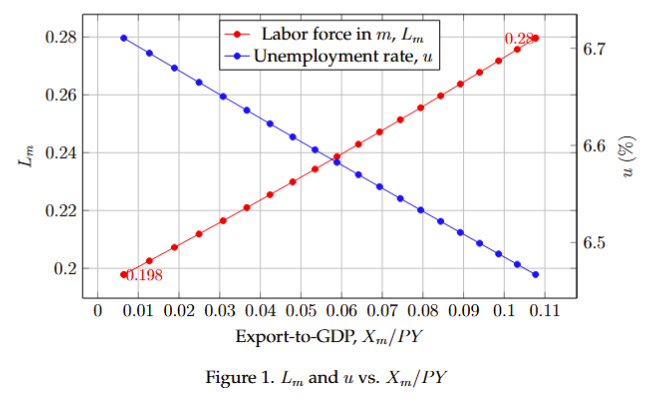
\includegraphics[width=0.8\textwidth]{openness.png}


\end{frame}


\begin{frame}{$\tau^{K*}$ + $\tau^{T*}$  vs. $\tau^{K*}$ only when $\beta= \eta$}

%Compared to SP,  "subsidy only" plans incur higher fiscal cost, less capital deepening, more vacancies/tighter labor market, and lower welfare.


\begin{itemize}
    

\item Optimal policy to replicate SP: 

Investment subsidy $\tau^{K*}_i$ financed by lump-sum fee $\tau^{T*}_i$ (DE1).

%investment subsidy can be in the form of CIT reduction (as CIT is mainly on capital income). 

%the lump-sum fee is proportional to firm size (employment).

\vspace{3mm}

\item Only implement $\tau^{K*}_i$ but set $\tau^T_i=0$ (DE2, DE3):

(i)  Fiscal cost $>0$

(ii) Lower welfare than SP, because  excessive vacancy creation leads to: 

--  $k_i< k_i^{SP}$, as vacancy filling rate too low

-- lower home production. 




\end{itemize}

\begin{table}[H]
% \caption{Equilibrium allocations under Taxes and Subsidies} \label{policytable}
\resizebox{\textwidth}{!}{
\centering
 \begin{tabular}{||c c c c||} 
 \hline
 \textbf{Moment} & \textbf{DE1}  & \textbf{DE2 }  & \textbf{DE3}\\  
 Description    & Replicates SP & Only $\tau^K$  & only uniform $\tau^K$ \\
  $\tau^K_i$  &   $\tau^K_i=\tau^{K*}_i$     &  $\tau^K_i=\tau^{K*}_i$    &  $\tau^K_i = \tau^{K*}_m$  \\
    $\tau^T_i$  &   $\tau^T_i=\tau^{T*}_i$     &  0    &   0  \\
 \hline\hline
  Industrial labor force, $L_m$   & 23.9\% & $24.5\%$   &   $23.9\%$ \\
  Industrial unemploy. rate, $u_m/L_m$ & 7.6\% & $6.9\%$  &  $6.9\%$  \\ 
   Services unemploy. rate, $u_s/L_s$  & 8.1\% &   $6.9\%$   &   $6.9\%$  \\ 
  Capital-to-output ratio, $K/Y$  & 3.4    & 3.3  &  3.2 \\
 % Tightness $\theta_m$  & 0.34  &  0.42  &  0.42  \\
 %   Tightness $\theta_s$  & 1.71 &  2.44  &  2.40 \\
 % Vacancy-filling rate $q_m$ & 1.72 &   1.54   &  1.55 \\
 %   Vacancy-filling rate $q_s$  & 0.76 &   0.64   &  0.65 \\
%  Total capital,  $K$  & 252  & 319 & $ + 27\% $\\
 % Relative prices, $p_s/p_m$ & 0.473  &  0.474 \\
%  Labor productivity, $A_m\f_m(k_m)/A_s\f_m(k_s)$ & 42.1 & 43.5 & $+3.3\% $\\ 
%  \textbf{Non-Targeted Moments} &  &  \\
% Relative wages, $w_m/w_s$ &  1.09 & 1.08 \\
 %Real output, $Y_m$    & 40.02    & 40.31  & $ 39.45\\
 %Real output, $Y_s$ &   2.69  &  2.66 & $ 2.60 \\
% Real consumption $C$ & 4.26  & 4.26  & 4.20  \\  
 Welfare, $W$  &     4.38    &  4.35      &  4.29                      \\
 Annual fiscal cost ($\%$ of GDP)  &   0   &  2.3  & 2.1 \\
 % Training Expenses/GDP & 0.75\% & 0.75\% \\ 
 \hline
 \end{tabular}}
%\end{adjustbox}
 
\end{table} 


    
\end{frame}


%\begin{frame}[allowframebreaks,noframenumbering]{References}
%  \bibliography{biblio}
%\end{frame}
%\end{document}

\end{document}